\chapter{Estado del Arte}
\label{chap:sota}

\lettrine{E}{n} este capítulo se ofrece una explicación del estado del arte sobre 
el uso de videojuegos como entorno de investigación en \gls{ia}, enfocándose especialmente en \textit{Minecraft}. 
Se describen los trabajos más relevantes en el ámbito de los videojuegos, haciendo especial énfasis
en aquellos que utilizan \textit{Minecraft} como entorno de experimentación.

Los juegos han sido un buen campo de prueba para el desarrollo de la \gls{ia}, 
gracias a su capacidad para simular entornos complejos e interactivos, y a la posibilidad de medir el 
rendimiento de los agentes de manera objetiva. 
Desde juegos clásicos con espacios de acción limitados, como el ajedrez~\cite{DBLP:journals/corr/abs-1712-01815}
o el \textit{Go}~\cite{DBLP:journals/nature/SilverHMGSDSAPL16}, que pese a disponer de un espacio de acciones reducido 
generan un espacio de estados prácticamente infinito, hasta juegos de estrategia en tiempo real con espacios de acciones enormes, 
como \textit{StarCraft}~\cite{DBLP:journals/nature/VinyalsBCMDCCPE19} o \textit{Dota 2}~\cite{DBLP:journals/corr/abs-1912-06680},
con un número de estados casi imposible de explorar.

La temática común entre estos artículos es el uso del \gls{rl} (clásico o profundo) para entrenar agentes
que puedan competir a nivel humano o superarlo. A diferencia de los juegos de mesa mencionados anteriormente, que
se basan en turnos, ejemplos como \textit{Space Invaders}
o \textit{Pong} requieren una percepción visual y una respuesta rápida para interactuar con el entorno de forma óptima, 
lo que los convierte en un campo de prueba excelente para el \gls{drl},
con las \gls{dqn}~\cite{DBLP:journals/nature/MnihKSRVBGRFOPB15} como una de las primeras aproximaciones significativas en mezclar
refuerzo clásico con aprendizaje profundo.

\section{Técnicas de IA en Videojuegos}
Entre los enfoques aplicados a videojuegos, el \gls{drl} ha producido resultados destacables. 
Las redes \gls{dqn} alcanzaron un rendimiento comparable al
de jugadores humanos profesionales en un conjunto de \num{49} juegos de \textit{Atari}~\cite{DBLP:journals/nature/MnihKSRVBGRFOPB15},
\textit{AlphaStar} llegó a nivel Gran Maestro en \textit{StarCraft~II}~\cite{DBLP:journals/nature/VinyalsBCMDCCPE19}
y \textit{OpenAI Five} superó a equipos profesionales en \textit{Dota~2}~\cite{DBLP:journals/corr/abs-1912-06680}.
Su principal limitación es la necesidad de una gran cantidad de interacciones con el
entorno y el diseño de una función de recompensa correcta.

Por otra parte, las \gls{htn} han demostrado ser competitivas
en juegos de estrategia en tiempo real como \textit{StarCraft}~\cite{DBLP:conf/ijcai/OntanonB15},
produciendo comportamientos deterministas e interpretables sin necesidad de
entrenamiento, aunque a costa de requerir conocimiento del dominio codificado
manualmente.

Sin embargo, con la llegada de los \gls{transformer}~\cite{DBLP:conf/nips/VaswaniSPUJGKP17}, 
se han empezado a aplicar estas técnicas a la investigación en videojuegos con resultados 
prometedores~\cite{DBLP:conf/nips/BakerAZHTEHSC22, DBLP:journals/corr/abs-2305-16291, DBLP:conf/nips/FanWJMYZTHZA22, oasis2024}. 
Estas aproximaciones difieren entre sí: algunas emplean un \gls{llm} para generar directamente las acciones o el código que controla al agente 
en lugar de una red neuronal entrenada por refuerzo. 
En el caso de \textit{Voyager}~\cite{DBLP:journals/corr/abs-2305-16291}, el \gls{llm} genera código \textit{JavaScript}
para controlar a un agente en \textit{Minecraft} en función de su entorno. Otras, como \textit{Oasis}~\cite{oasis2024},
emplean el \gls{transformer} como modelo generativo para construir un clon interactivo de \textit{Minecraft}.

\section{Minecraft como Entorno de Investigación}
Actualmente existen diversos trabajos relacionados con el uso de \textit{Minecraft} como
entorno de investigación en \gls{ia},
como el proyecto \textit{MineRL}~\cite{guss2019minerl}, que proporciona un conjunto de datos y un
entorno de simulación para entrenar agentes \gls{rl} en \textit{Minecraft}.

En esta misma línea, \textit{MineDojo}~\cite{DBLP:conf/nips/FanWJMYZTHZA22} amplía el enfoque con un
conjunto masivo de tareas abiertas y una extensa base de conocimiento multimodal extraída de Internet (vídeos, \textit{wiki} y foros).

En el ámbito de los \gls{llm}, \textit{Mindcraft}~\cite{mindcraft2025} es un \gls{mas} basado en \gls{llm} para el razonamiento colaborativo,
en el que los agentes generan código \textit{JavaScript} para actuar en \textit{Minecraft}, de forma similar al enfoque empleado por
\textit{Voyager}~\cite{DBLP:journals/corr/abs-2305-16291}, cuya arquitectura se muestra en la Figura~\ref{fig:Voyager} (página~\pageref{fig:Voyager}).
El objetivo a largo plazo de estos sistemas es completar el juego de forma totalmente autónoma, sin intervención humana.

\begin{figure}[htbp]
  \centering
  \resizebox{\textwidth}{!}{
  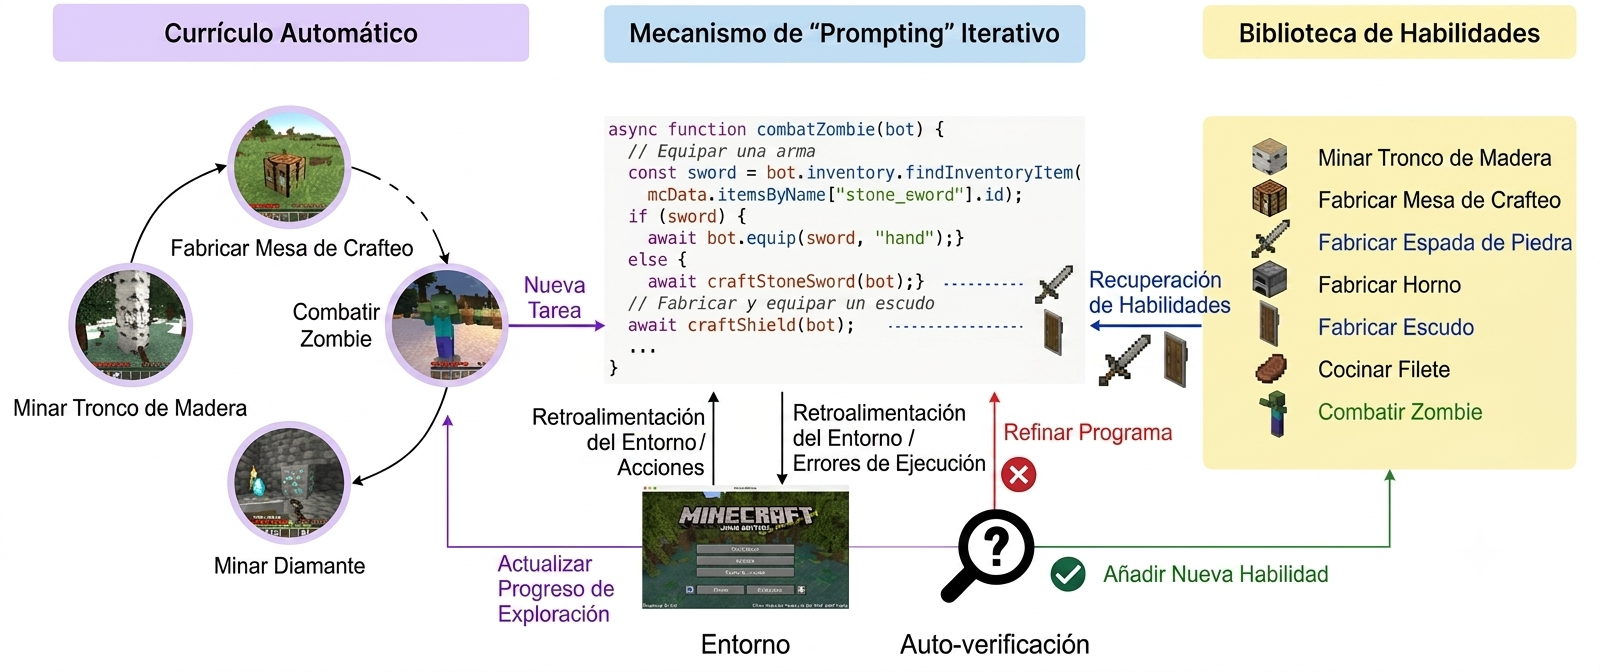
\includegraphics[width=1\textwidth]{imaxes/02_sota/voyager.png}
  }
  \caption[Arquitectura del agente Voyager]{Arquitectura de \textit{Voyager}~\cite{DBLP:journals/corr/abs-2305-16291},
  un sistema basado en \gls{llm} para controlar un agente en \textit{Minecraft}. El \gls{llm} genera código \textit{JavaScript} para controlar
  al agente en función de su entorno y construye de forma incremental una biblioteca de habilidades reutilizables.}
  \label{fig:Voyager}
\end{figure}

\section{Técnicas de IA aplicadas a Minecraft}
\subsection{Aprendizaje por Imitación}
El referente de \gls{il} en \textit{Minecraft} es \gls{vpt}~\cite{DBLP:conf/nips/BakerAZHTEHSC22},
que preentrena una \gls{política} sobre \num{70000} horas de vídeo sin etiquetar,
logrando comportamientos complejos por imitación. Su limitación
principal es el desajuste entre los estados del experto y los que explora el
aprendiz (\gls{distribution-shift}). Para mitigarlo, \gls{dagger}~\cite{DBLP:journals/jmlr/RossGB11} 
emplea al experto sobre los estados recorridos para corregir los errores cometidos por el aprendiz,
aunque el artículo original no se implementó en \textit{Minecraft}.

\subsection{Aprendizaje por Refuerzo}
En \textit{Minecraft}, la complejidad y ambigüedad de las recompensas, junto con los largos horizontes temporales, 
incrementan tanto el coste como la dificultad del entrenamiento. Dentro de estas aproximaciones, los enfoques que
alcanzan un buen rendimiento dependen de recursos difíciles de replicar en \textit{hardware} común: 
\gls{vpt}~\cite{DBLP:conf/nips/BakerAZHTEHSC22} se apoya en un preentrenamiento masivo sobre decenas de 
miles de horas de vídeo, y un \gls{world-model}
como \textit{DreamerV3}~\cite{DBLP:journals/corr/abs-2301-04104} requiere entrenamientos muy prolongados
para resolver tareas de horizonte largo. Como respuesta a este coste, la competición \textit{MineRL}~\cite{guss2019minerl} surgió
para incentivar la eficiencia muestral, y trabajos como el de
Scheller et al.~\cite{DBLP:journals/corr/abs-2003-06066}
mostraron que incorporar demostraciones humanas reduce el número de
interacciones necesarias, aunque sin eliminar por completo la
dependencia de cómputo.